\documentclass[10pt]{beamer}

\mode<presentation>{% Settings
    % link to view http://www.hartwork.org/beamer-theme-matrix/
    % ------------------------------------------------------------------------------
    % Slide Themes
    % ------------------------------------------------------------------------------
    %\usetheme{default}
    %\usetheme{AnnArbor}
    %\usetheme{Antibes}
    %\usetheme{Bergen}
    \usetheme{Berkeley}
    %\usetheme{Berlin}
    %\usetheme{Boadilla}
    %\usetheme{CambridgeUS}
    %\usetheme{Copenhagen}
    %\usetheme{Darmstadt}
    %\usetheme{Dresden}
    %\usetheme{Frankfurt}
    %\usetheme{Goettingen}
    %\usetheme{Hannover}
    %\usetheme{Ilmenau}
    %\usetheme{JuanLesPins} % rounded title, gradient at top with section, no bottom bar
    %\usetheme{Luebeck}     % square title, toc at top of each slide
    %\usetheme{Madrid}      % rounded title
    %\usetheme{Malmoe}
    %\usetheme{Marburg}
    %\usetheme{Montpellier}
    %\usetheme{PaloAlto}
    %\usetheme{Pittsburgh}
    %\usetheme{Rochester}
    %\usetheme{Singapore}
    %\usetheme{Szeged}
    %\usetheme{Warsaw}

    % ------------------------------------------------------------------------------
    % Color Schemes
    % ------------------------------------------------------------------------------
    %\usecolortheme{default}
    %\usecolortheme{albatross}  % blue background with darker blue
    %\usecolortheme{beaver}     % gray with red
    %\usecolortheme{beetle}     % gray background
    %\usecolortheme{crane}      % orange
    \usecolortheme{dolphin}     % white with purple
    %\usecolortheme{dove}       % all white
    %\usecolortheme{fly}        % all gray including background
    %\usecolortheme{lily}       % white with blue
    %\usecolortheme{orchid}     % default blue
    %\usecolortheme{rose}       % default blue
    %\usecolortheme{seagull}    % darker gray than seahorse
    %\usecolortheme{seahorse}   % light gray blueish tint
    %\usecolortheme{whale}      % default blue
    %\usecolortheme{wolverine}  % yellow with a little blue

    %\setbeamertemplate{footline} % To remove the footer line in all slides uncomment this line
    %\setbeamertemplate{footline}[page number] % To replace the footer line in all slides with a simple slide count uncomment this line
    \setbeamertemplate{navigation symbols}{} % To remove the navigation symbols from the bottom of all slides uncomment this line
    \setbeamertemplate{bibliography item}{\insertbiblabel} % to number bibliography entries
}

\usepackage{Logemann}
\usepackage{Integral}
\usepackage{Derivative}
\usepackage{Sum}
\usepackage{SetTheory}
\usepackage[backend=biber]{biblatex}
\addbibresource{refs.bib}

\title[]{Introduction to Discontinuous Galerkin Methods} % The short title
% appears at the bottom of every slide, the full title is only on the title page

\author{Caleb Logemann} % Your name
\institute[Iowa State University]{% Your institution as it will appear on the bottom of every slide, may be shorthand to save space
Mathematics Department, Iowa State University \\ % Your institution for the title page
\medskip
\textit{logemann@iastate.edu}} % Your email address

\date{November 10, 2017} % Date, can be changed to a custom date

\begin{document}
  \begin{frame}
    \titlepage{}
  \end{frame}

  \begin{frame}
    \frametitle{Goal}
    \begin{itemize}
      \item Numerically Solve
        \begin{align*}
          u_t + f(u)_x = 0 \\
          x \in \Omega \subset \RR^d \qquad t \in \RR^+
        \end{align*}

      \item Weak Solution
        Find $u$ such that for any test function $v$
        \[
          \dintt{0}{\infty}{\dintt{\RR^d}{}{u_t v + f(u)_x v}{x}}{t} = 0
        \]
    \end{itemize}
  \end{frame}

  \begin{frame}
    \frametitle{Goal}
    \begin{itemize}
      \item Numerically Solve
        \begin{align*}
          u_t + f(u)_x = 0 \\
          x \in \br{a, b} \quad t \in \RR^+
        \end{align*}

      \item Weak Solution
        Find $u$ such that for any test function $v$
        \[
          \dintt{0}{\infty}{\dintt{a}{b}{u_t v + f(u)_x v}{x}}{t} = 0
        \]
    \end{itemize}
  \end{frame}

  \begin{frame}
    \frametitle{Generate Mesh}
    \begin{itemize}
      \item 1D Uniform Grid
          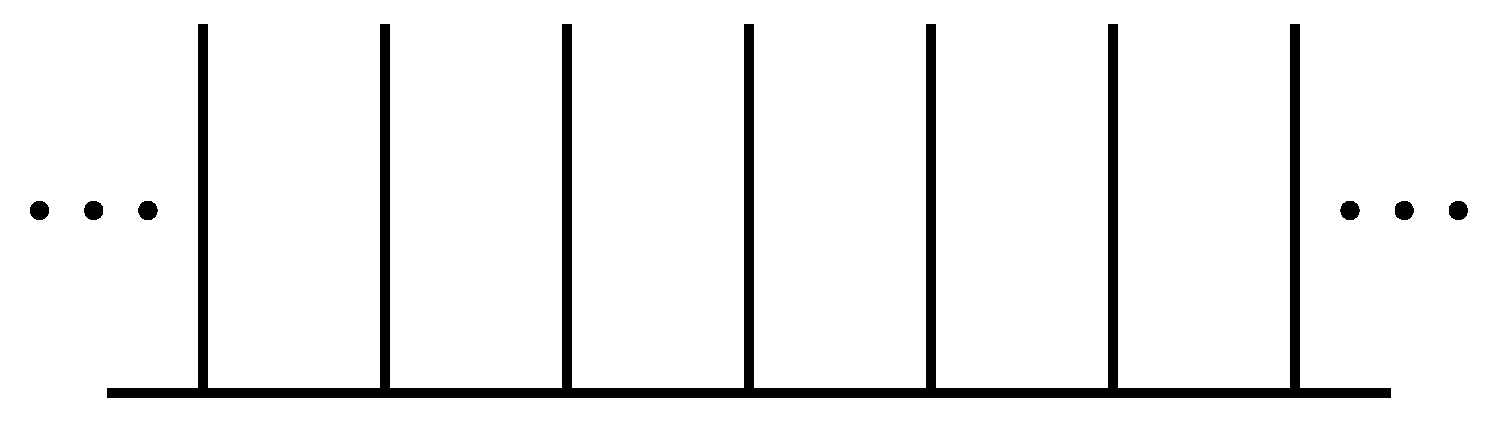
\includegraphics[scale=0.3]{Figures/1Dgrid}
      \item 1D Variable Grid
          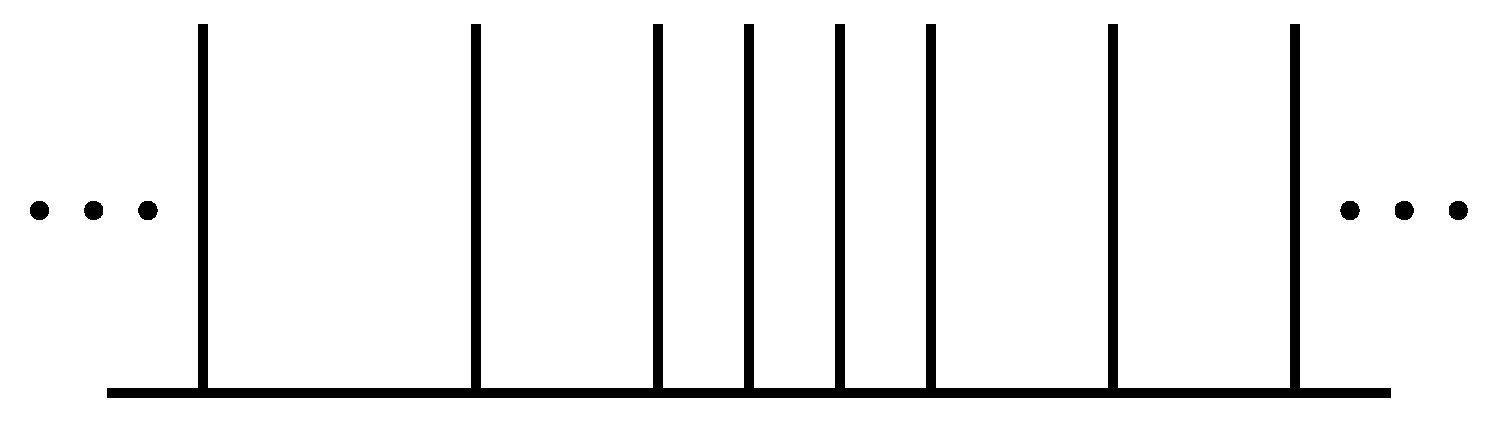
\includegraphics[scale=0.3]{Figures/1Dgrid_nonuniform}
    \end{itemize}
  \end{frame}

  \begin{frame}
    \frametitle{Generate Mesh}
    \begin{itemize}
      \item 2D Uniform Grid \hfill \\
          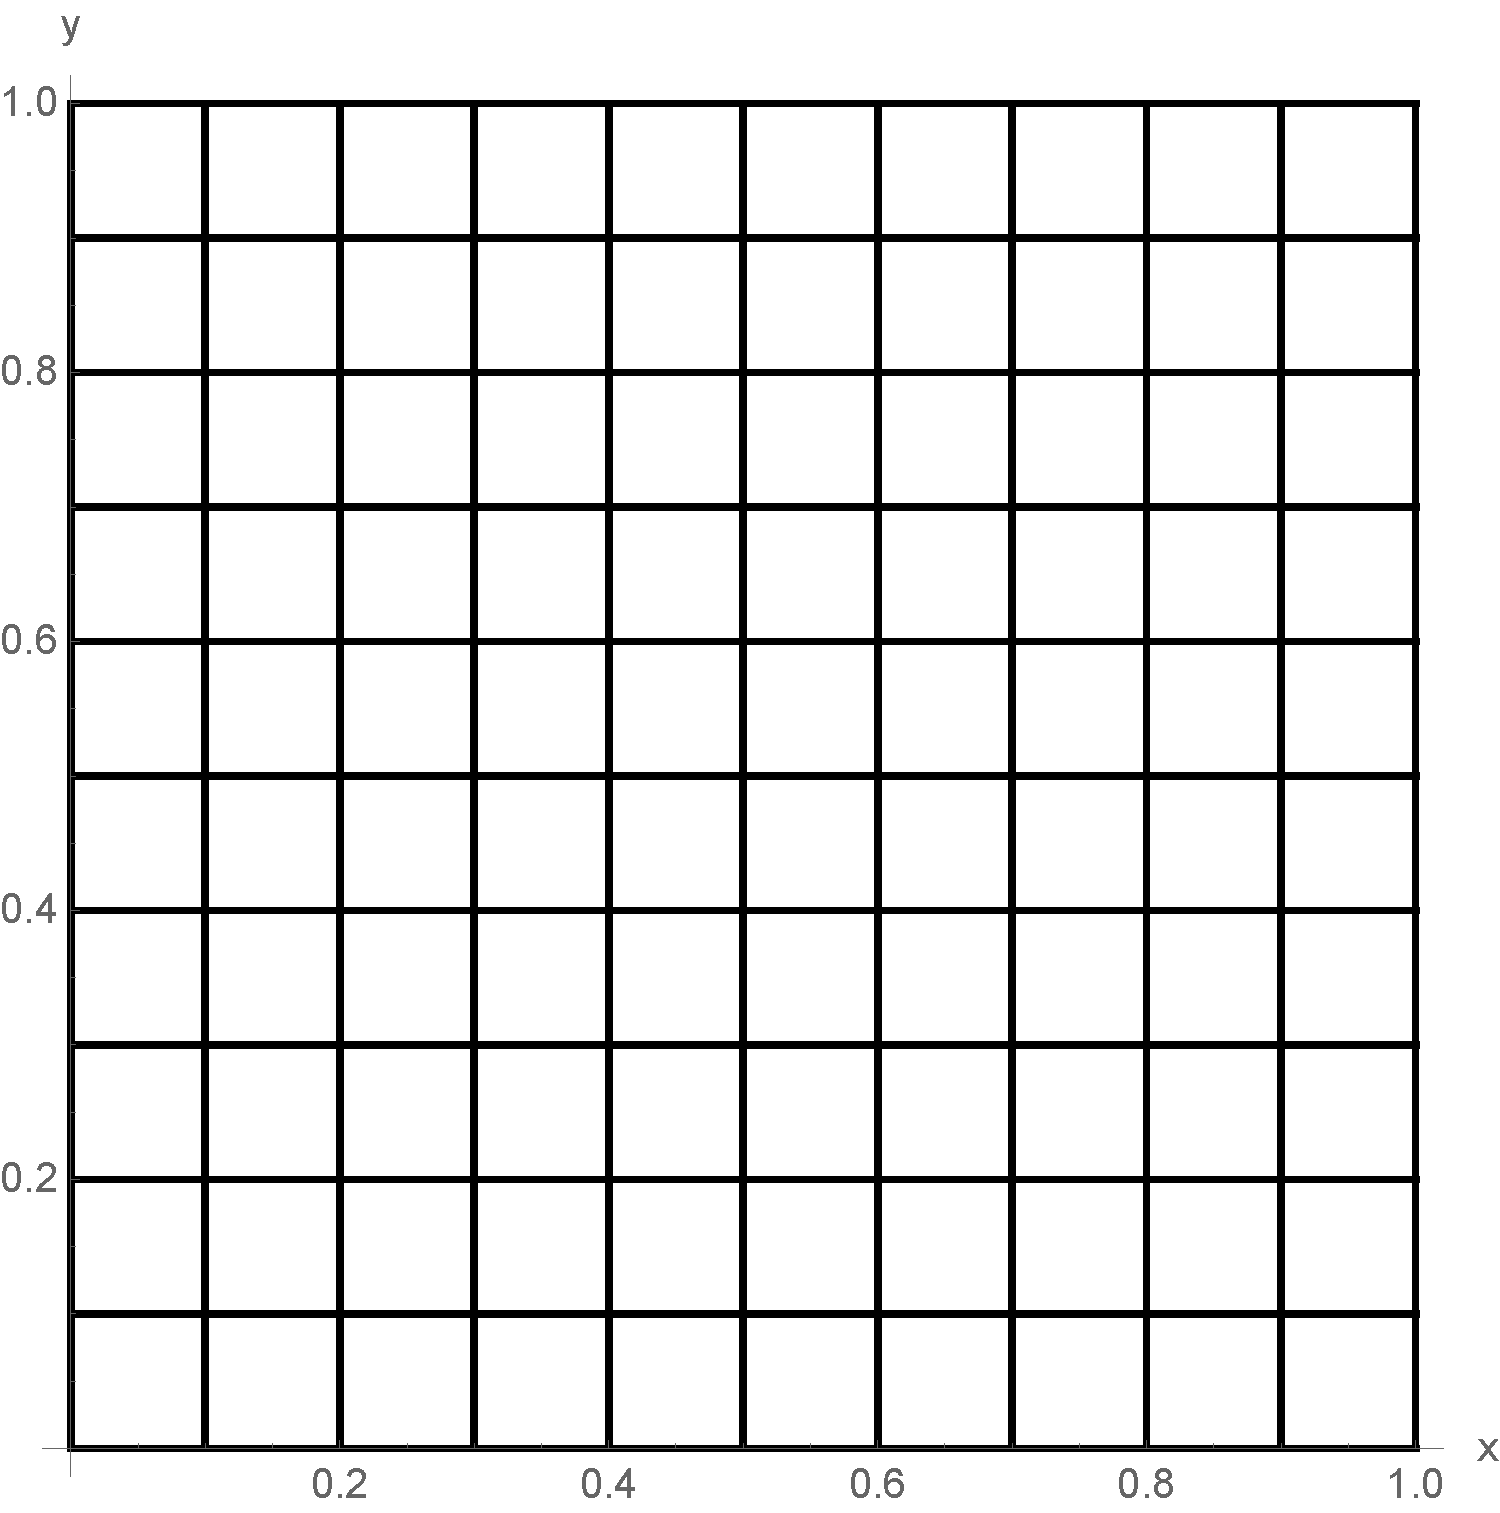
\includegraphics[scale=0.27]{Figures/2Dgrid}
    \end{itemize}
  \end{frame}

  \begin{frame}
    \frametitle{Generate Mesh}
    \begin{itemize}
      \item 2D Unstructured Triangulation
          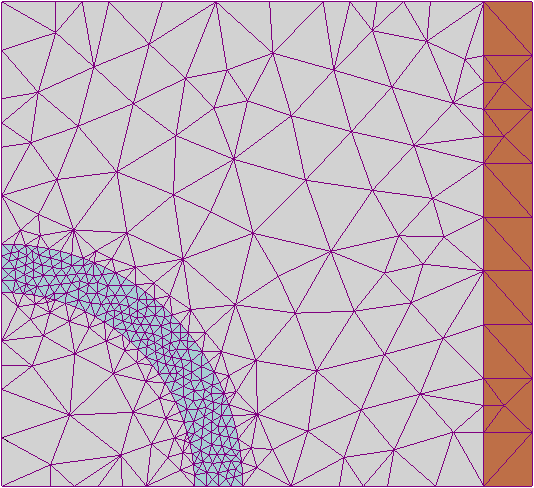
\includegraphics[scale=0.4]{Figures/2Dmesh}
    \end{itemize}
  \end{frame}

  \begin{frame}
    \frametitle{Generate Mesh}
    \begin{itemize}
      \item 3D Unstructured Triangulation
          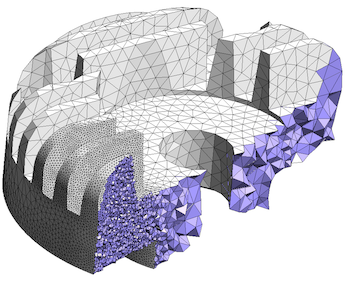
\includegraphics[scale=0.6]{Figures/3Dmesh}
    \end{itemize}
  \end{frame}

  \begin{frame}
    \frametitle{Generate Mesh}
    \begin{itemize}
      \item 3D Unstructured Triangulation
          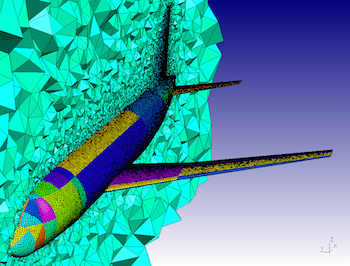
\includegraphics[scale=0.6]{Figures/3Dmesh2}
    \end{itemize}
  \end{frame}

  \begin{frame}
    \frametitle{Solution Space}
    \begin{itemize}
      \item Label each element in mesh as $I_j$, $j = 1, \ldots N$
      \item Discontinuous Galerkin Finite Element Space
        \[
          V^M = \set{u: \eval{u}{I_j}{} \in P^M(I_j), j = 1, \ldots, N}
        \]

        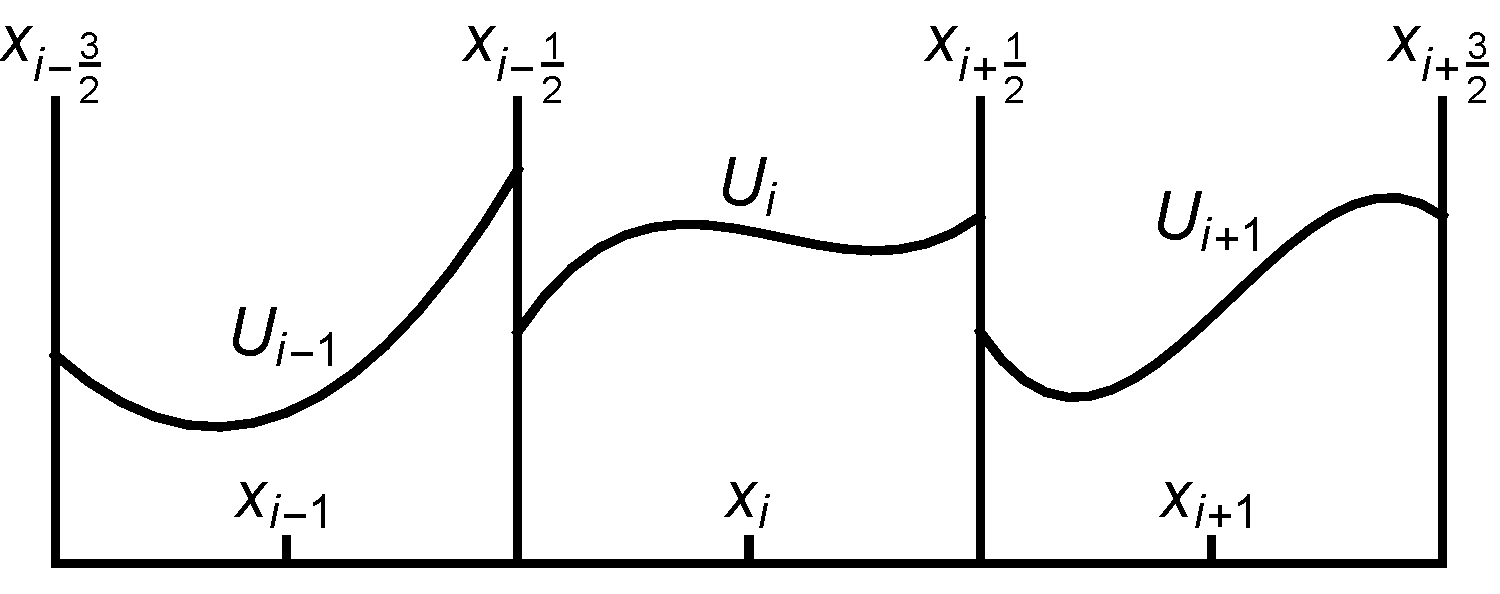
\includegraphics[scale=0.35]{Figures/DG.pdf}
    \end{itemize}
  \end{frame}

  \begin{frame}
    \frametitle{The Method}
    \begin{itemize}
      \item At a given time find $u \in V^M$ such that for all $v \in V^M$ and for all $j = 1, \ldots, N$.
        \[
          \dintt{I_j}{}{u_t v}{x} + \dintt{I_j}{}{f(u)_x v}{x} = 0
        \]

      \item Integrate by parts
        \[
          \dintt{I_j}{}{u_t v}{x} + \hat{f}_{j+1/2} v^-_{j+1/2} - \hat{f}_{j-1/2} v^+_{j-1/2} - \dintt{I_j}{}{f(u) v_x}{x} = 0
        \]

      \item $\hat{f}$ is called the numerical flux
        \begin{itemize}
          \item Consistent: $\hat{f}{u, u}$
        \end{itemize}
    \end{itemize}
  \end{frame}

  \begin{frame}
    \frametitle{Numerical Flux}
    \begin{itemize}
      \item Approximating $f(u(x_{j+1/2}, t))$
        \[
          \hat{f}_{j+1/2} = \hat{f}(u_{j+1/2}^-, u_{j+1/2}^+)
        \]

      \item Properties
        \begin{itemize}
          \item Consistent: $\hat{f}(u, u) = f(u)$
          \item Lipschitiz Continuous with respect to both arguments
          \item Monotone: non-decreasing in first argument, non-increasing with second argument
        \end{itemize}

      \item Examples
        \begin{itemize}
          \item Godunov
            \[
              \hat{f}_{j+1/2} =
              \begin{cases}
                \min[u \in \br{u^-, u^+}]{f(u)} & u^- < u^+ \\
                \max[u \in \br{u^+, u^-}]{f(u)} & u^- \ge u^+ \\
              \end{cases}
            \]

          \item Rusanov/Local Lax-Friedrichs
            \[
              \hat{f}(u^-, u^+) = \frac{1}{2}\p{f(u^-) + f(u^+) - \alpha(u^+ - u^-)}
            \]
            where $\alpha = \max[u]{\abs{f'(u)}}$.
        \end{itemize}
    \end{itemize}
  \end{frame}

  \begin{frame}
    \frametitle{Implementation}
    \begin{itemize}
      \item Linear transformation $x \in \br{x_{j-1/2}, x_{j+1/2}}$ to $\xi \in \br{-1, 1}$
        \[
          x = \frac{\Delta x}{2} \xi + \frac{x_{j-1/2} + x_{j+1/2}}{2}
        \]
        \[
          \xi = \frac{2}{\Delta x} \p{x - \frac{x_{j-1/2} + x_{j+1/2}}{2}}
        \]

      \item Pick a basis for $P^M(\br{-1,1})$, e.g. Legendre polynomials
        \[
          \frac{1}{2}\dintt{-1}{1}{\phi^j(\xi) \phi^k(\xi)}{\xi} = \delta_{jk}
        \]
        \[
          \phi^1(\xi) = 1 \qquad \phi^2(\xi) = \xi \qquad \phi^3(\xi) = \sqrt{5}/2(3\xi^2 - 1)
        \]
    \end{itemize}
  \end{frame}

  \begin{frame}
    \frametitle{Implementation}
    \begin{itemize}
      \item Galerkin Expansion
        \[
          \eval{u}{I_j}{} = \sum{k = 1}{M}{U_k \phi^k(\xi)}
        \]

      \item Let $v = \phi^j$
        \begin{align*}
          \dintt{-1}{1}{u_t \phi^j}{\xi} + \frac{2}{\Delta x}\p{\hat{f}_{j+1/2} \phi^j(1) - \hat{f}_{j-1/2} \phi^j(-1)} \\
          - \frac{2}{\Delta x}\dintt{-1}{1}{f(u) \phi^j_{\xi}}{\xi} = 0
        \end{align*}
      \item Using the orthonormality
        \begin{align*}
          \p{U_k}_t = \frac{1}{\Delta x}\dintt{-1}{1}{f(u) \phi^j_{\xi}}{\xi} - \frac{1}{\Delta x}\p{\hat{f}_{j+1/2} \phi^j(1) - \hat{f}_{j-1/2} \phi^j(-1)}
        \end{align*}
    \end{itemize}
  \end{frame}

  \begin{frame}
    \frametitle{Solving the ODE}
    
    \begin{itemize}
      \item General ODE
        \[
          U_t = L(U)
        \]

      \item Forward Euler
        \[
          U^{n+1} = U^n + L(U^n)
        \]

      \item Backward Euler
        \[
          U^{n+1} = U^n + L(U^{n+1})
        \]

      \item Higher Order Explicit or Implicit Runge-Kutta Schemes
    \end{itemize}
  \end{frame}

  \begin{frame}
    \frametitle{Ongoing Research}
    \begin{itemize}
      \item Create DG methods for certain types of equations
      \item Slope/Oscillation Limiting
      \item Strong Stability Preserving (SSP)
      \item Entropy Solutions
      \item Positivity Preserving
    \end{itemize}
  \end{frame}

  \section{Introduction}
    \begin{frame}
      \frametitle{Motivation}
      \begin{itemize}
        \item Aircraft Icing
        \item Runback
      \end{itemize}
      \begin{center}
        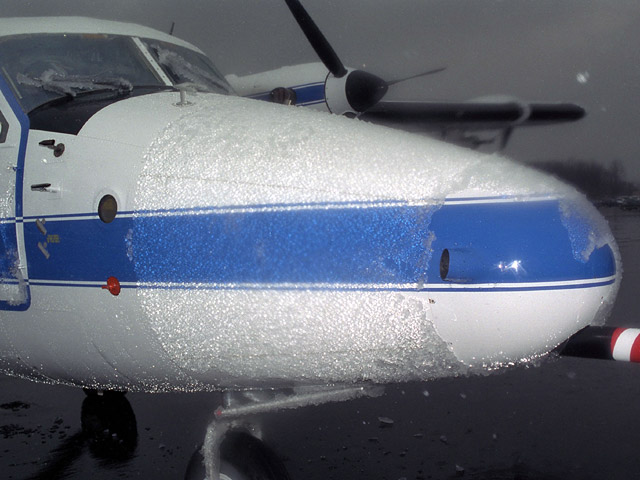
\includegraphics[scale=0.2]{Figures/Icing_on_a_plane.jpg}
        \hspace{0.1in}
        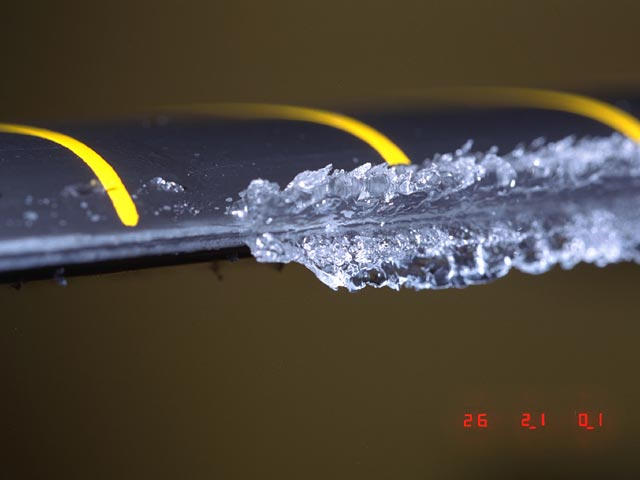
\includegraphics[scale=0.2]{Figures/Icing_on_a_rotor.jpg}
      \end{center}
      \begin{itemize}
        \item Industrial Coating
        \item Paint Drying
      \end{itemize}
    \end{frame}

    \begin{frame}
      \frametitle{Model Equations}
      \begin{itemize}
        \item Navier-Stokes Equation
          \begin{align*}
            \rho_t + \p{\rho u}_x &= 0 \\
            \p{\rho u}_t + \p{\rho u^2 + p}_x &=  \frac{4}{3Re} u_{xx} \\
            E_t + \p{u (E + p)}_x &= \frac{1}{Re} \p{\frac{2}{3} \p{u^2}_{xx} + \frac{\gamma}{(\gamma - 1)Pr} \p{\frac{p}{\rho}}_{xx}}
          \end{align*}
        \item Asymptotic Limit, $\rho << L$
        \item Thin-Film Equation - 1D with $u$ as fluid height.
          \[
            u_t + \p{f(x, t) u^2 - g(x, t) u^3}_x = -\p{h(x, t) u^3 u_{xxx}}_x
          \]
      \end{itemize}
    \end{frame}

    \begin{frame}
      \frametitle{Current Model}
      \begin{itemize}
        \item Simplified Expression
          \[
            u_t + \p{u^2 - u^3}_x = -\p{u^3 u_{xxx}}_x
          \]

        \item Operator Splitting
          \begin{align*}
            u_t + \p{u^2 - u^3}_x &= 0 \\
            u_t + \p{u^3 u_{xxx}}_x &= 0
          \end{align*}
      \end{itemize}
    \end{frame}


    \begin{frame}
      \frametitle{Numerical Solutions}
      \begin{itemize}
        \item Use canonical variable $\xi \in \br{-1, 1}$
        \item Let $\set{\phi^k(\xi)}$ be the Legendre polynomials.

        \item Solution of order $M$ on each cell
          \[
            \eval{u}{x \in V_i}{} \approx U_i = \sum*{k = 1}{M}{U_i^k \phi^k(\xi)}
          \]
          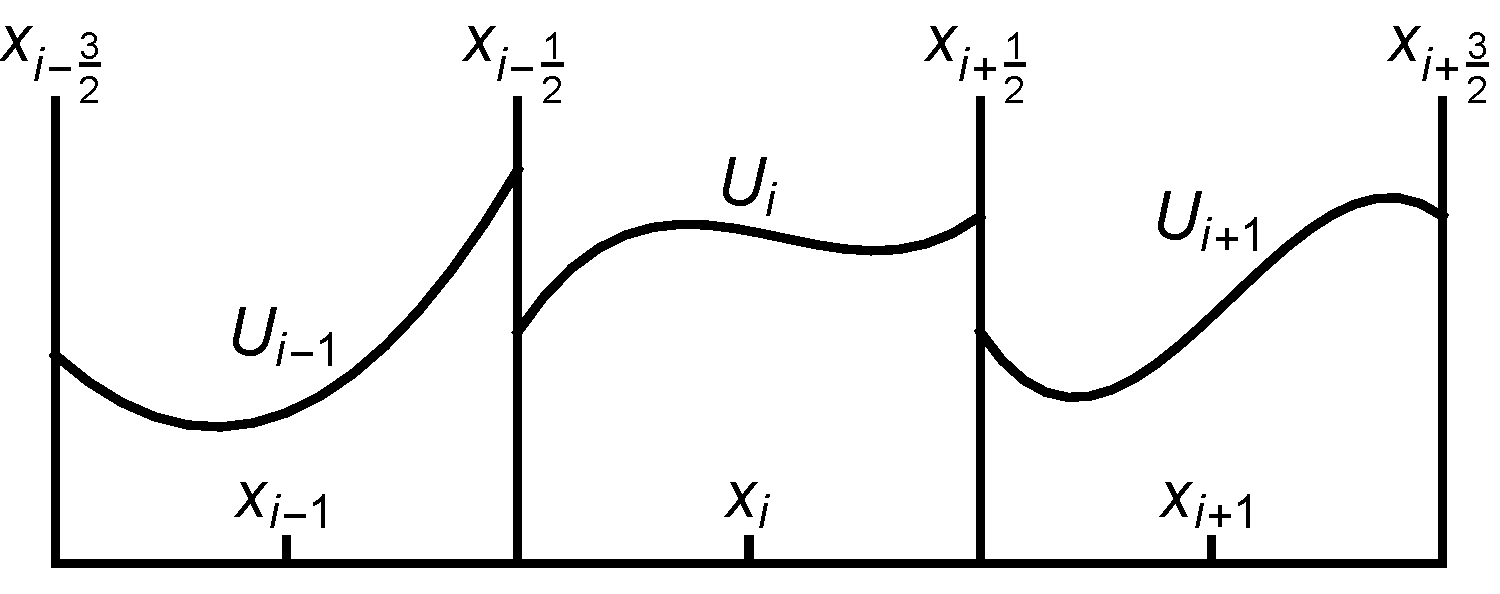
\includegraphics[scale=0.35]{Figures/DG.pdf}
      \end{itemize}
    \end{frame}

  \section{Convection}
    \begin{frame}
      \frametitle{Convection}
      \begin{itemize}
        \item Convection Equation
          \begin{gather*}
            u_t + \frac{2}{\Delta x} f(u)_\xi = 0 \\
            f(u) = u^2 - u^3
          \end{gather*}

        \item Weak Form
          \[
            \dintt*{-1}{1}{u_t \phi(\xi) + \frac{2}{\Delta x}f(u)_\xi \phi(\xi)}{\xi} = 0
          \]

        \item Runge-Kutta Discontinuous Galerkin
          %\[
            %\dintt{-1}{1}{\p{U_i}_t \phi^{\ell}(\xi)}{\xi} - \dintt{-1}{1}{\frac{2}{\Delta x}\p{\p{U_i}^2 - \p{U_i}^3} \phi^{\ell}_{\xi}(\xi)}{\xi} + \frac{2}{\Delta x}\p{\mcF_{i + 1/2} \phi^{\ell}(1) - \mcF_{i - 1/2} \phi^{\ell}(-1)} = 0
          %\]
          \[
            \dot{U_i^{\ell}} = \frac{1}{\Delta x}\dintt{-1}{1}{f(U_i)\phi_{\xi}^{\ell}}{\xi} - \frac{1}{\Delta x} \p{\mcF_{i + 1/2} - \mcF_{i - 1/2}}
          \]

        \item Rusanov Numerical Flux
          \[
            \mcF_{j+1/2} = \frac{f\p{U_{i+1}(-1)} + f\p{U_{i}(1)}}{2} \phi^{\ell}(1)
          \]

        \item Solve this system of ODEs with any Explicit Strong Stability Preserving (SSP) Runge-Kutta Method.
      \end{itemize}
    \end{frame}

    \begin{frame}
      \frametitle{Numerical Example - Square Wave}
      \begin{center}
        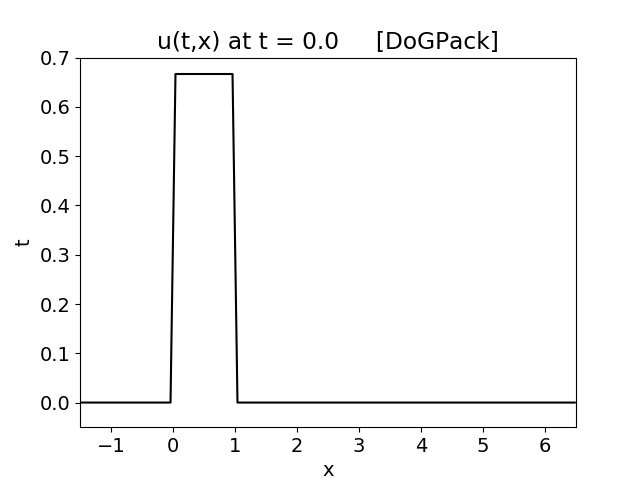
\includegraphics[scale=0.6]{Figures/squarewave00.png}
      \end{center}
    \end{frame}
    \begin{frame}
      \frametitle{Numerical Example - Square Wave}
      \begin{center}
        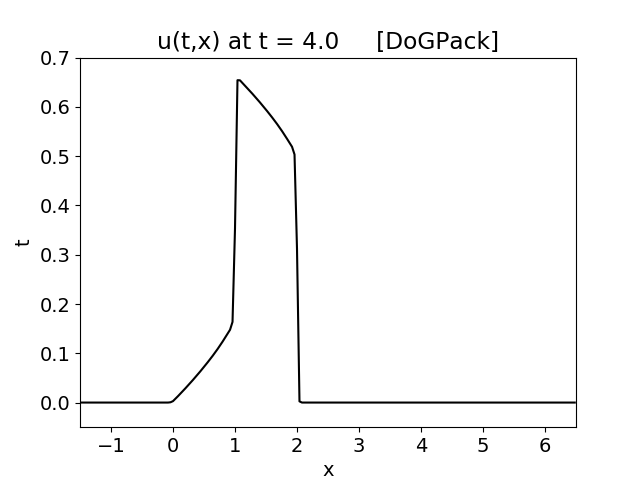
\includegraphics[scale=0.6]{Figures/squarewave04.png}
      \end{center}
    \end{frame}
    \begin{frame}
      \frametitle{Numerical Example - Square Wave}
      \begin{center}
        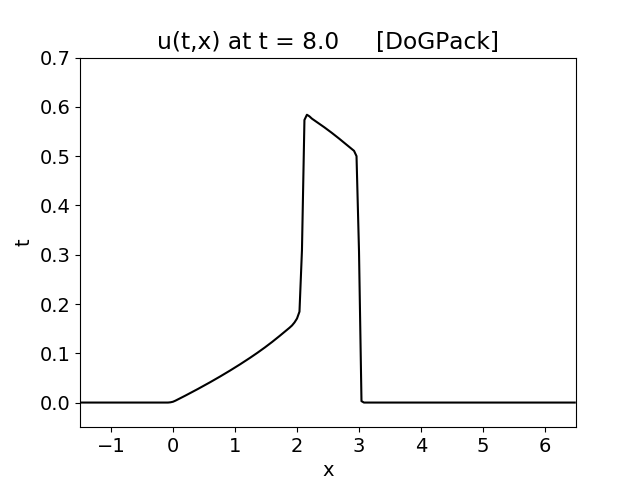
\includegraphics[scale=0.6]{Figures/squarewave08.png}
      \end{center}
    \end{frame}
    \begin{frame}
      \frametitle{Numerical Example - Square Wave}
      \begin{center}
        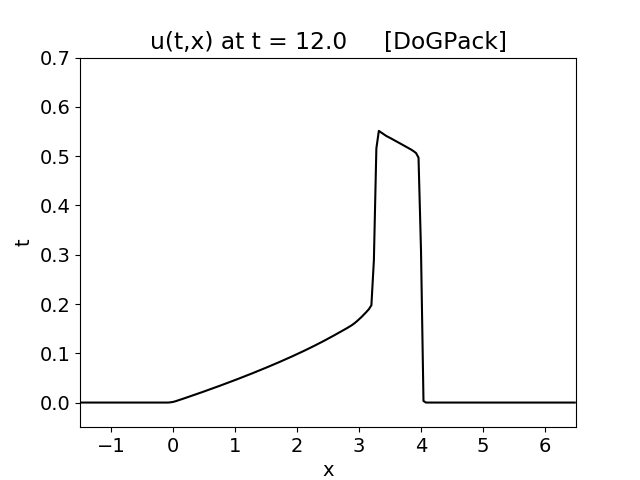
\includegraphics[scale=0.6]{Figures/squarewave12.png}
      \end{center}
    \end{frame}
    \begin{frame}
      \frametitle{Numerical Example - Square Wave}
      \begin{center}
        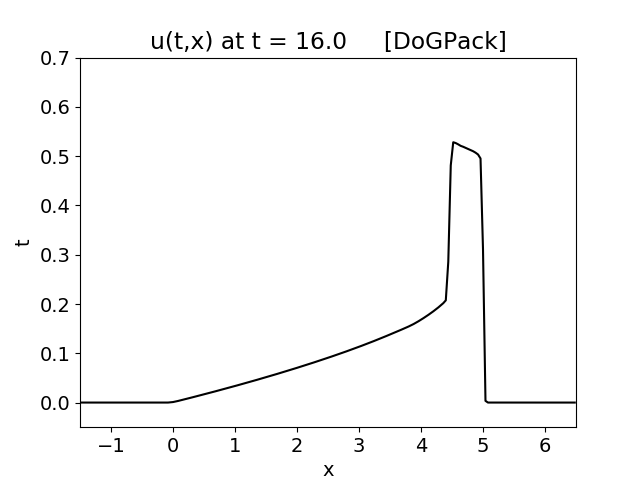
\includegraphics[scale=0.6]{Figures/squarewave16.png}
      \end{center}
    \end{frame}
    \begin{frame}
      \frametitle{Numerical Example - Square Wave}
      \begin{center}
        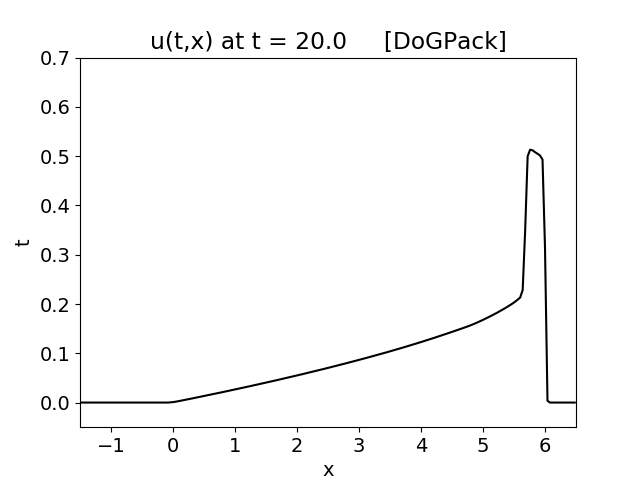
\includegraphics[scale=0.6]{Figures/squarewave20.png}
      \end{center}
    \end{frame}

  \section{Hyper-Diffusion}
    \begin{frame}
      \frametitle{Hyper-Diffusion}
      \begin{itemize}
        \item Hyper-Diffusion Equation
          \[
            u_t + \frac{16}{\Delta x^4} \p{u^3 u_{\xi\xi\xi}}_\xi = 0
          \]

        \item Local Discontinuous Galerkin (LDG)
          \begin{align*}
            q &= \frac{2}{\Delta x} u_{\xi} \\
            r &= \frac{2}{\Delta x} q_{\xi} \\
            s &= \frac{2}{\Delta x} u^3 r_{\xi} \\
            u_t &= -\frac{2}{\Delta x} s_{\xi}
          \end{align*}
      \end{itemize}
    \end{frame}

    \begin{frame}
      \frametitle{Local Discontinuous Galerkin}
      \begin{align*}
        \eta(\xi) &= \p{U_i^{n}}^3 \\
        Q_i^{\ell} &= -\frac{1}{\Delta x} \p{\dintt{-1}{1}{U_i \phi_{\xi}^{\ell}}{\xi}
        - \mcF(U)_{i+1/2}^{\ell} + \mcF(U)_{i - 1/2}^{\ell}} \\
        R_i^{\ell} &= -\frac{1}{\Delta x} \p{\dintt{-1}{1}{Q_i \phi_{\xi}^{\ell}}{\xi}
        - \mcF(Q)_{i+1/2}^{\ell} + \mcF(Q)_{i - 1/2}^{\ell}} \\
        S_i^{\ell} &= \frac{1}{\Delta x} \p{\dintt{-1}{1}{(R_i)_{\xi} \eta(\xi) \phi^{\ell}}{\xi}} \\
        &+ \frac{1}{\Delta x}\p{\mcF(\eta)_{i + 1/2} \mcF(R)_{i+1/2}^{\ell} - \mcF(\eta)_{i-1/2} \mcF(R)_{i-1/2}^{\ell}}\\
        \dot{U}_i^{\ell} &= \frac{1}{\Delta x} \p{\dintt{-1}{1}{S_i \phi_{\xi}^{\ell}}{\xi}
        - \mcF(S)_{i+1/2}^{\ell} + \mcF(S)_{i - 1/2}^{\ell}}
      \end{align*}
    \end{frame}

    \begin{frame}
      \frametitle{Local Discontinuous Galerkin}
      \begin{align*}
        \mcF(\eta)_{i+1/2} &= \frac{1}{2}\p{\eta_{i+1}(-1) - \eta_{i}(1)} \\
        \mcF(\eta)_{i-1/2} &= \frac{1}{2}\p{\eta_{i-1}(1) - \eta_{i}(-1)} \\
        \mcF(*)_{i+1/2}^{\ell} &= \phi^{\ell}(1) *_{i+1/2}
      \end{align*}
      \begin{center}
        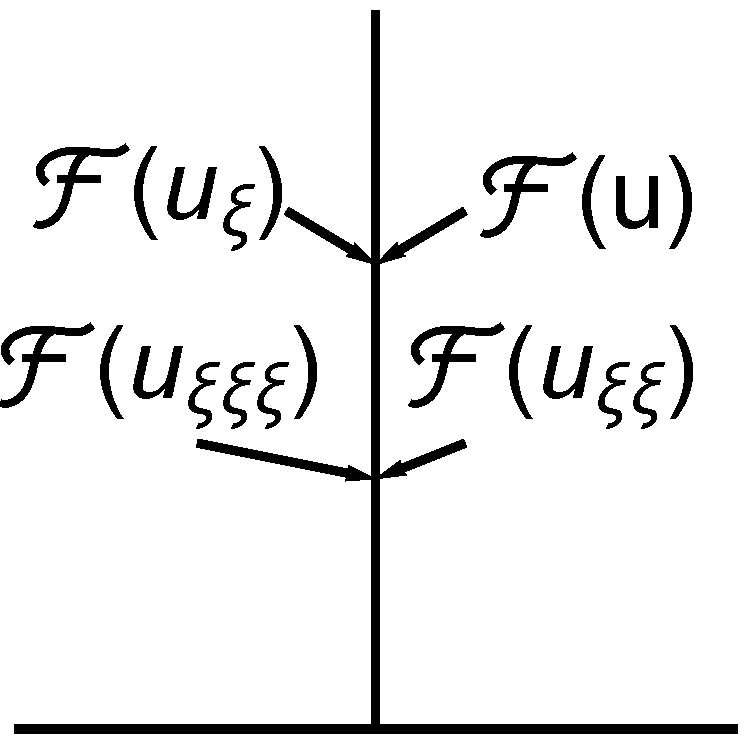
\includegraphics[scale=0.3]{Figures/localDG.pdf}
      \end{center}
    \end{frame}

    \begin{frame}
      \frametitle{Local Discontinuous Galerkin}
      \begin{itemize}
        \item Explicit SSP Runge Kutta
          \begin{itemize}
            \item Severe time step restriction
            \item $\Delta t \sim \Delta x^4$
            \item $\Delta x = .1 \to \Delta t \approx 10^{-4}$
            \item $\Delta x = .01 \to \Delta t \approx 10^{-8}$
          \end{itemize}

        \item Implicit SSP Runge Kutta
          \begin{itemize}
            \item Linear System Solver
            \item Stabilized BiConjugate Gradient
            \item MultiGrid Solver
          \end{itemize}
      \end{itemize}
    \end{frame}

    %\begin{frame}
      %\frametitle{Linear Solver}
      %\begin{itemize}
        %\item Stabilized BiConjugate Gradient
        %\item MultiGrid Solver \hfill \\

      %\end{itemize}
    %\end{frame}

    \begin{frame}
      \frametitle{Multigrid Solver}
      \begin{itemize}
        \item Relaxation e.g. Jacobi Relaxation
      \end{itemize}
      \begin{center}
        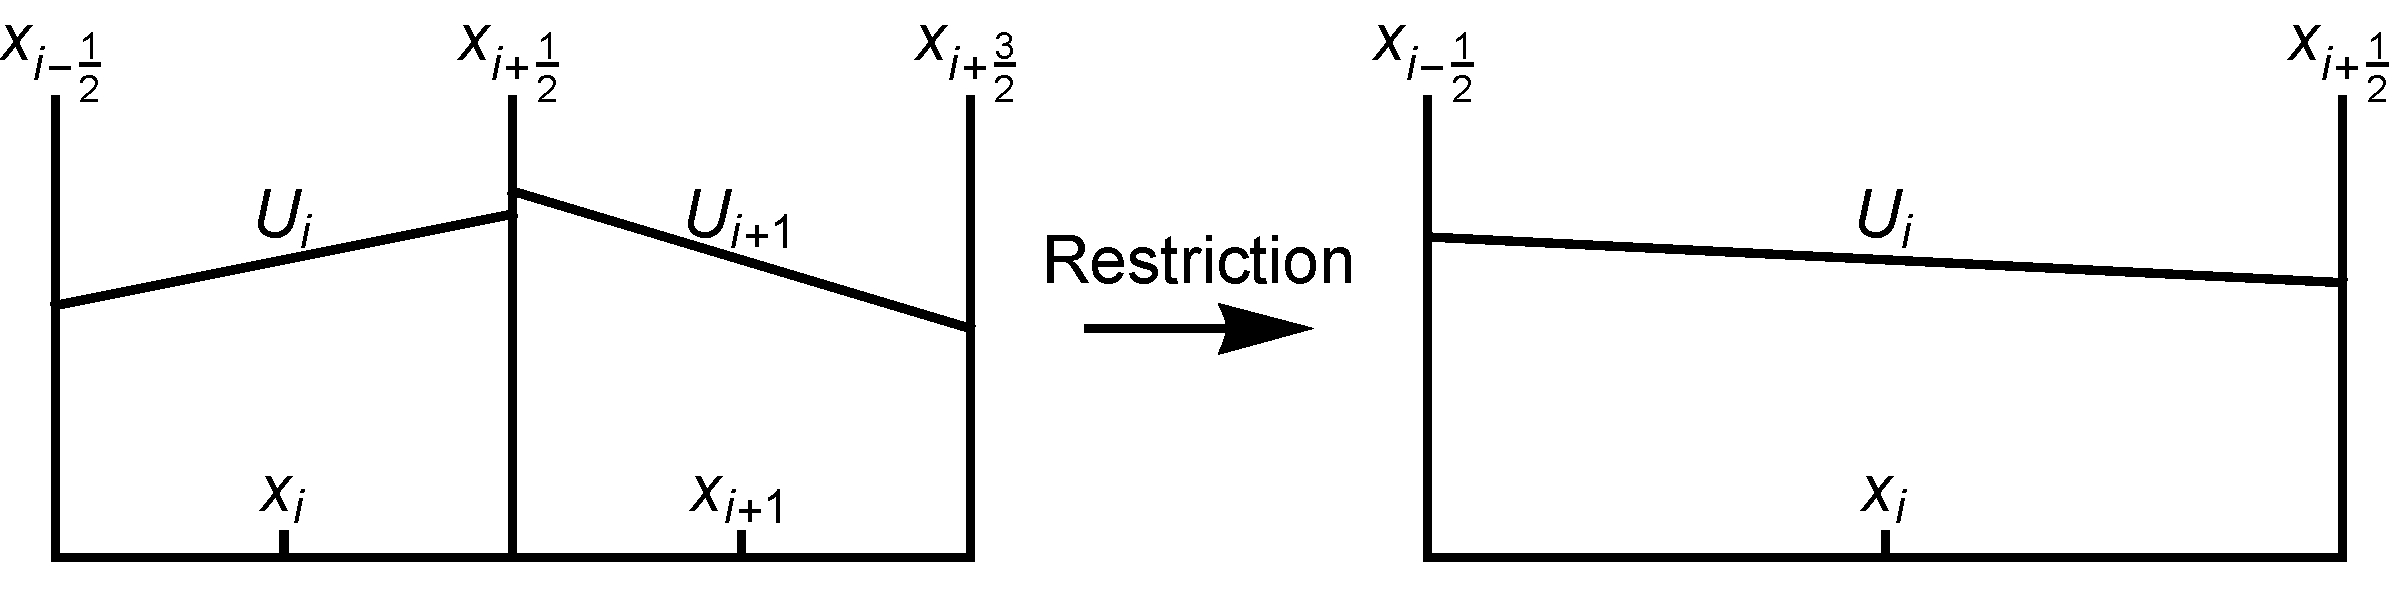
\includegraphics[scale=0.25]{Figures/restriction.pdf} \\
        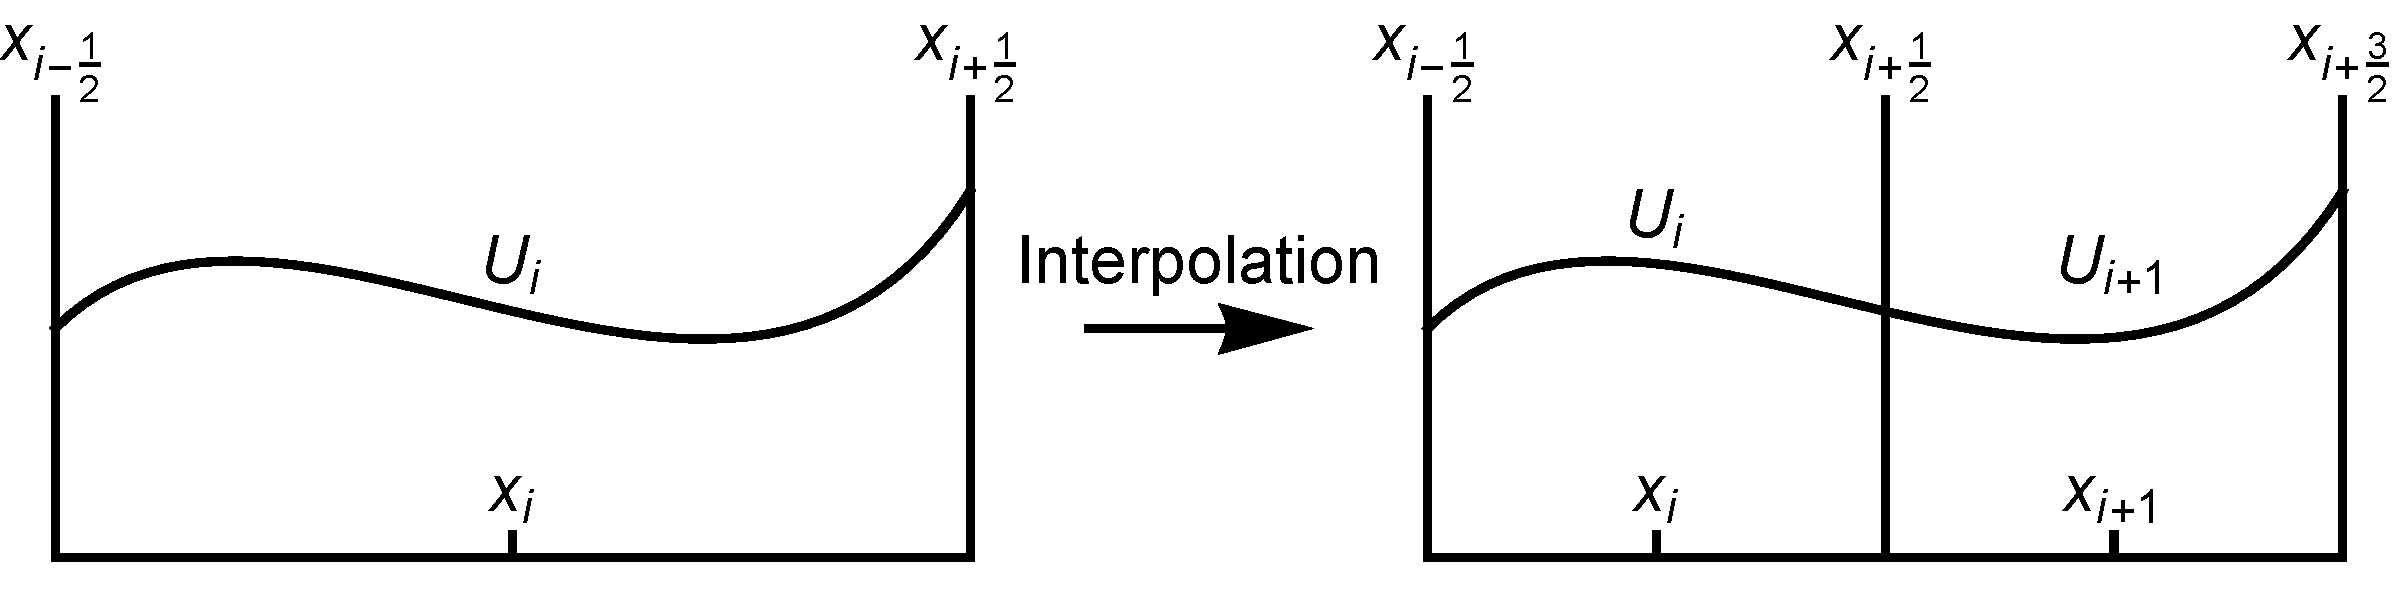
\includegraphics[scale=0.25]{Figures/interpolation.pdf}
      \end{center}
    \end{frame}

    \begin{frame}
      \frametitle{Multigrid Solver}
      V-Cycle
      \begin{center}
        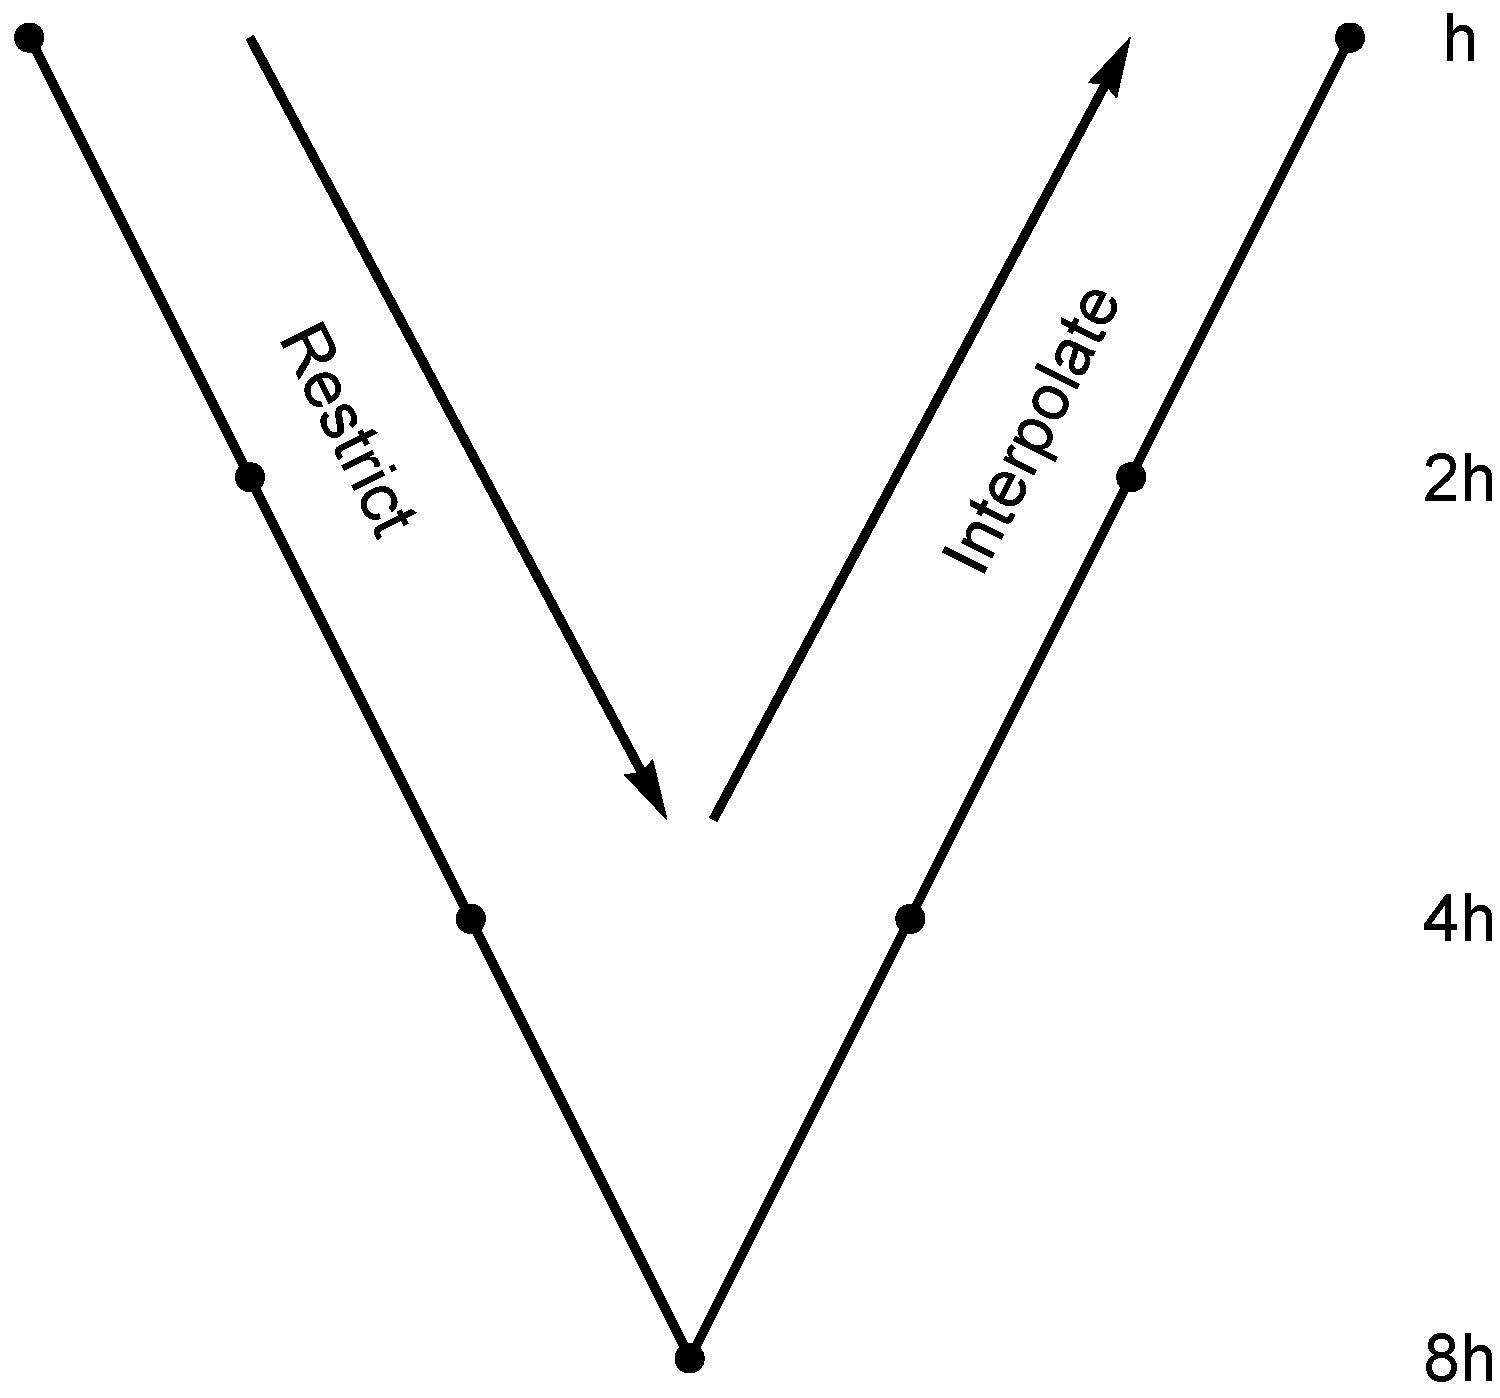
\includegraphics[scale=0.25]{Figures/vcycle.pdf}
      \end{center}
    \end{frame}

    \begin{frame}
      \frametitle{Multigrid Solver}
      \begin{center}
        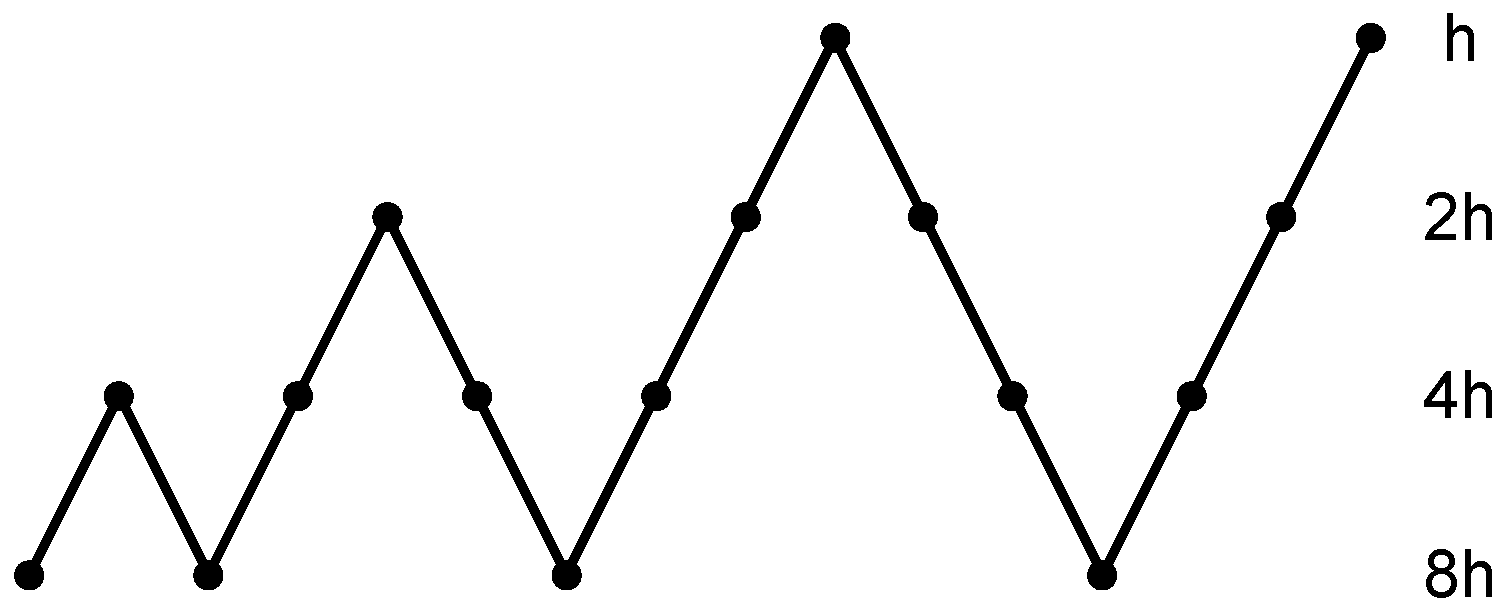
\includegraphics[scale=0.35]{Figures/mucycle.pdf}
      \end{center}
    \end{frame}

  \section{Operator Splitting}
    \begin{frame}
      \frametitle{Operator Splitting}
      \begin{itemize}
        \item Strang Splitting
          \begin{itemize}
            \item 1 time step
              \begin{itemize}
                \item 1/2 time step for convection
                \item 1 time step for hyper-diffusion
                \item 1/2 time step for convection
              \end{itemize}
            \item Second order splitting
          \end{itemize}
      \end{itemize}
    \end{frame}

    \begin{frame}
      \frametitle{Numerical Results - Riemann Problem}
      \begin{center}
        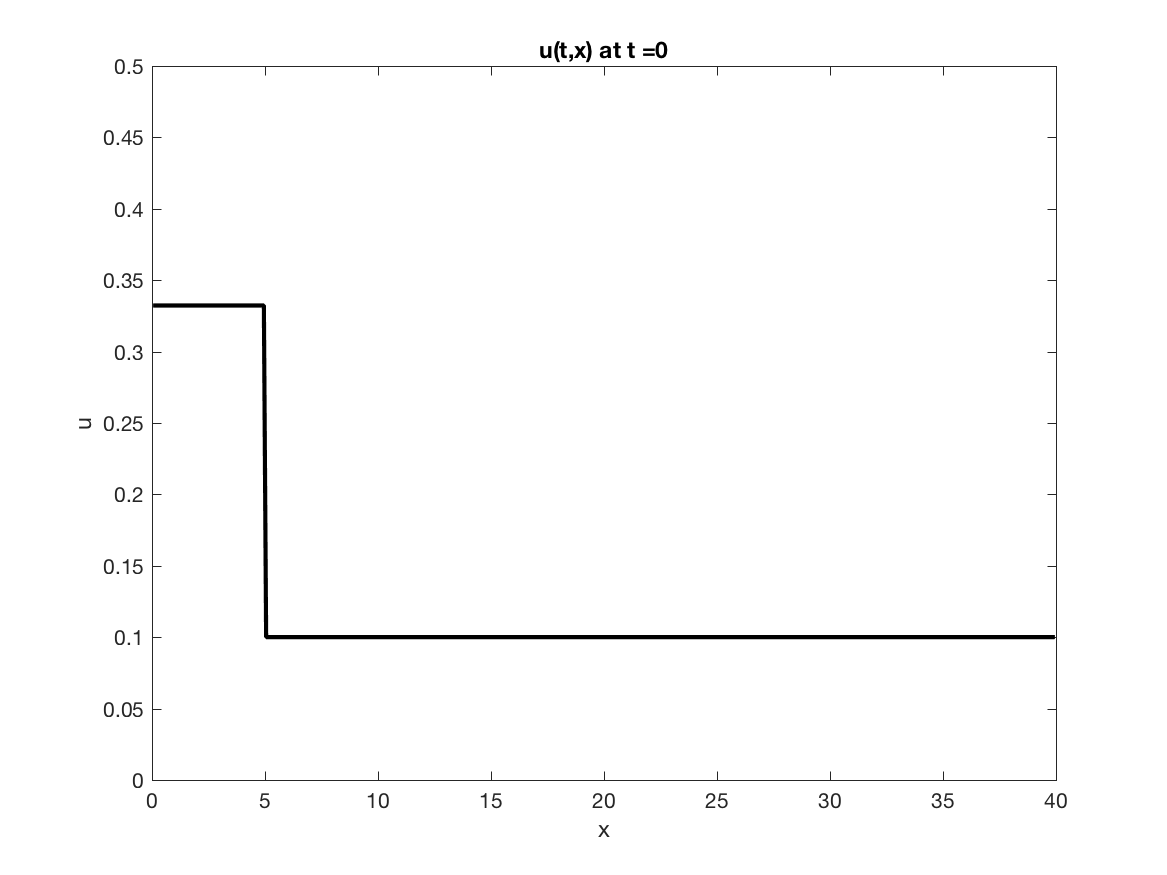
\includegraphics[scale=0.5]{Figures/reimann0.png}
      \end{center}
    \end{frame}
    \begin{frame}
      \frametitle{Numerical Results - Riemann Problem}
      \begin{center}
        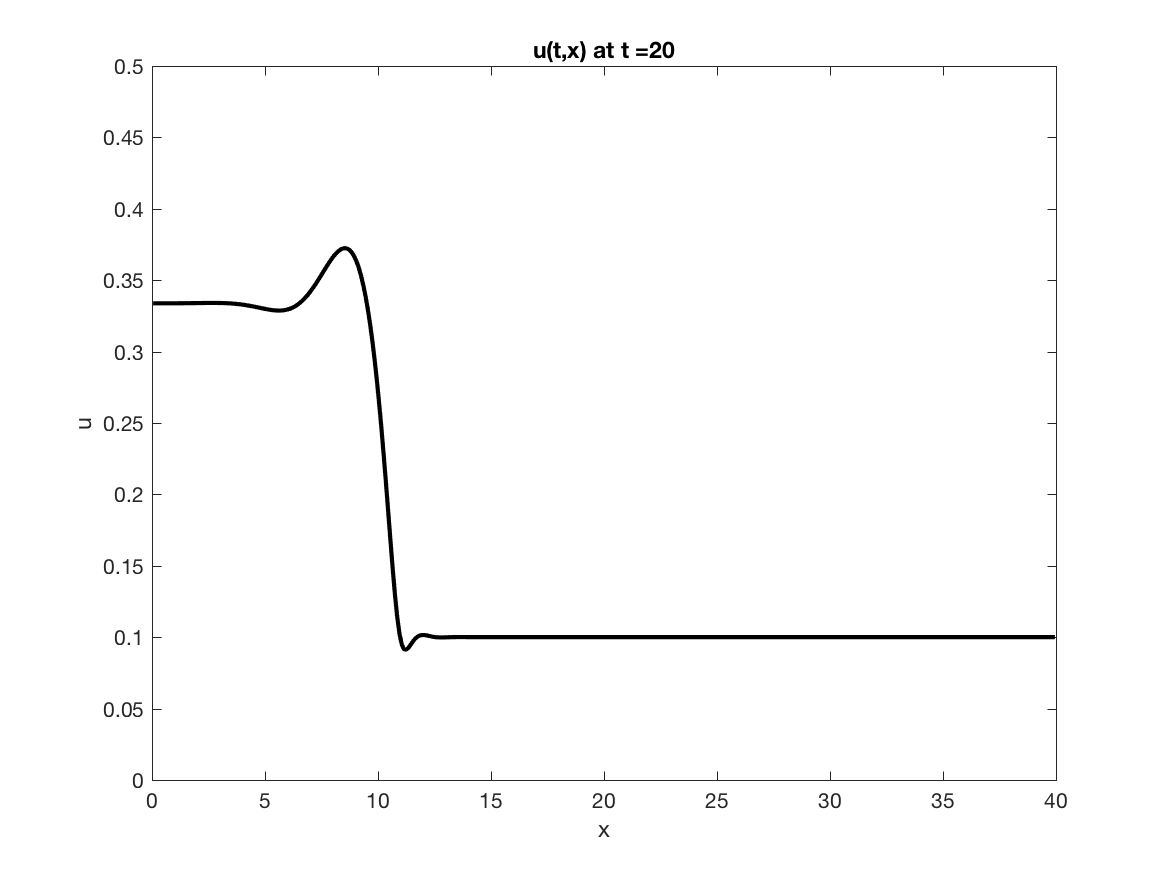
\includegraphics[scale=0.5]{Figures/reimann20.png}
      \end{center}
    \end{frame}
    \begin{frame}
      \frametitle{Numerical Results - Riemann Problem}
      \begin{center}
        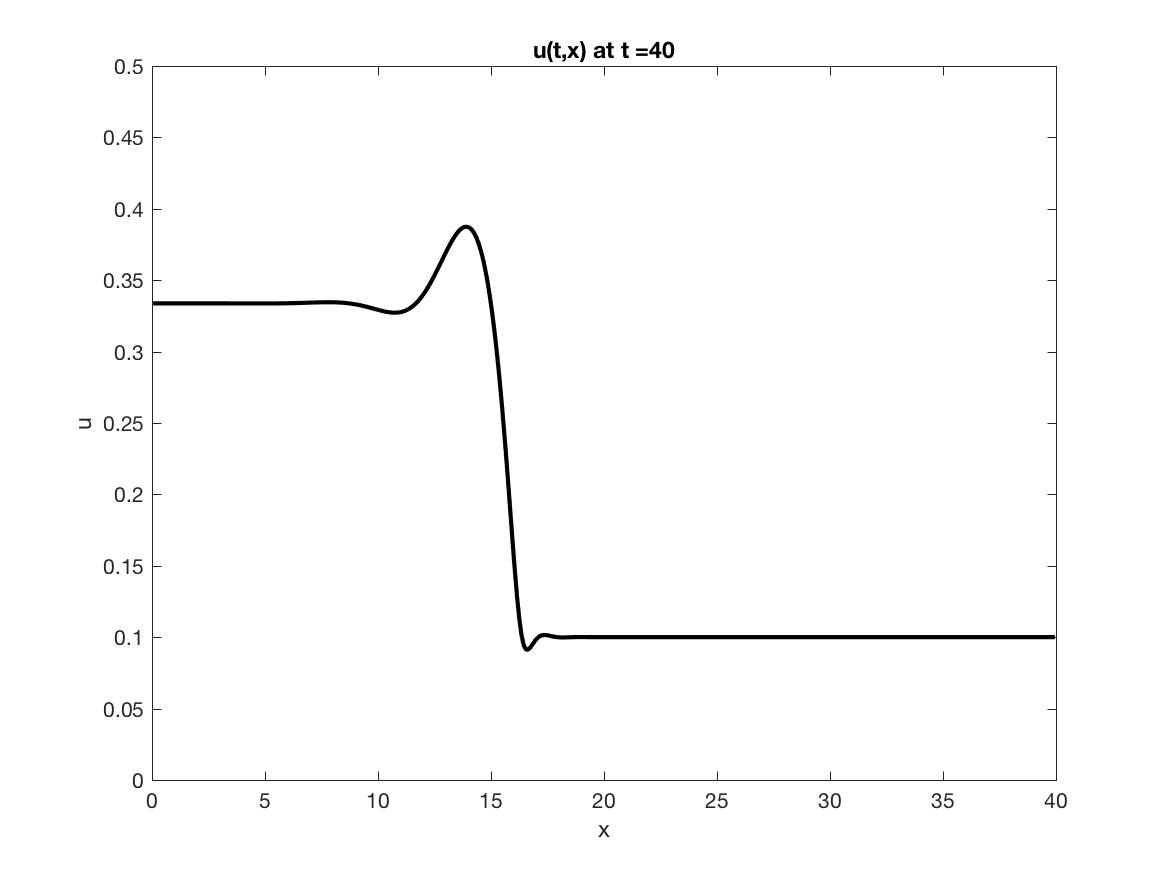
\includegraphics[scale=0.5]{Figures/reimann40.png}
      \end{center}
    \end{frame}
    \begin{frame}
      \frametitle{Numerical Results - Riemann Problem}
      \begin{center}
        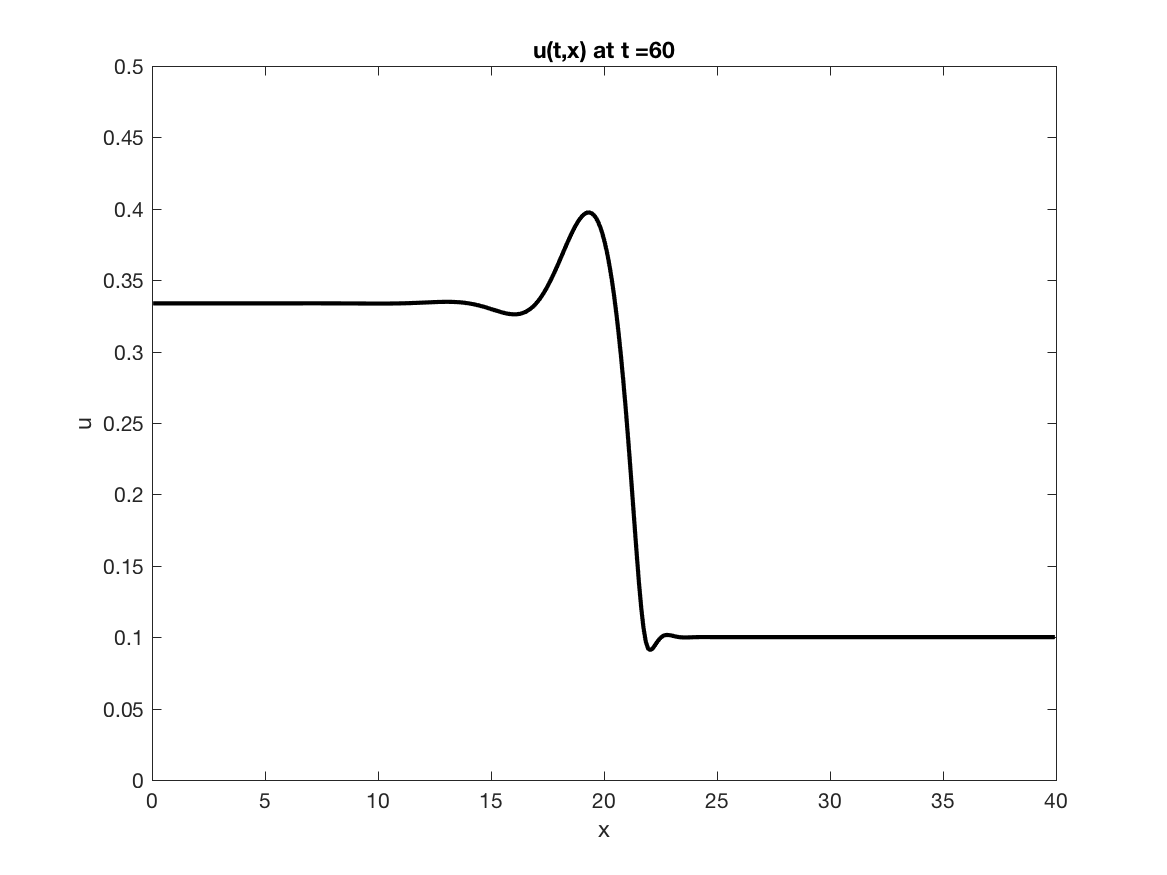
\includegraphics[scale=0.5]{Figures/reimann60.png}
      \end{center}
    \end{frame}
    \begin{frame}
      \frametitle{Numerical Results - Riemann Problem}
      \begin{center}
        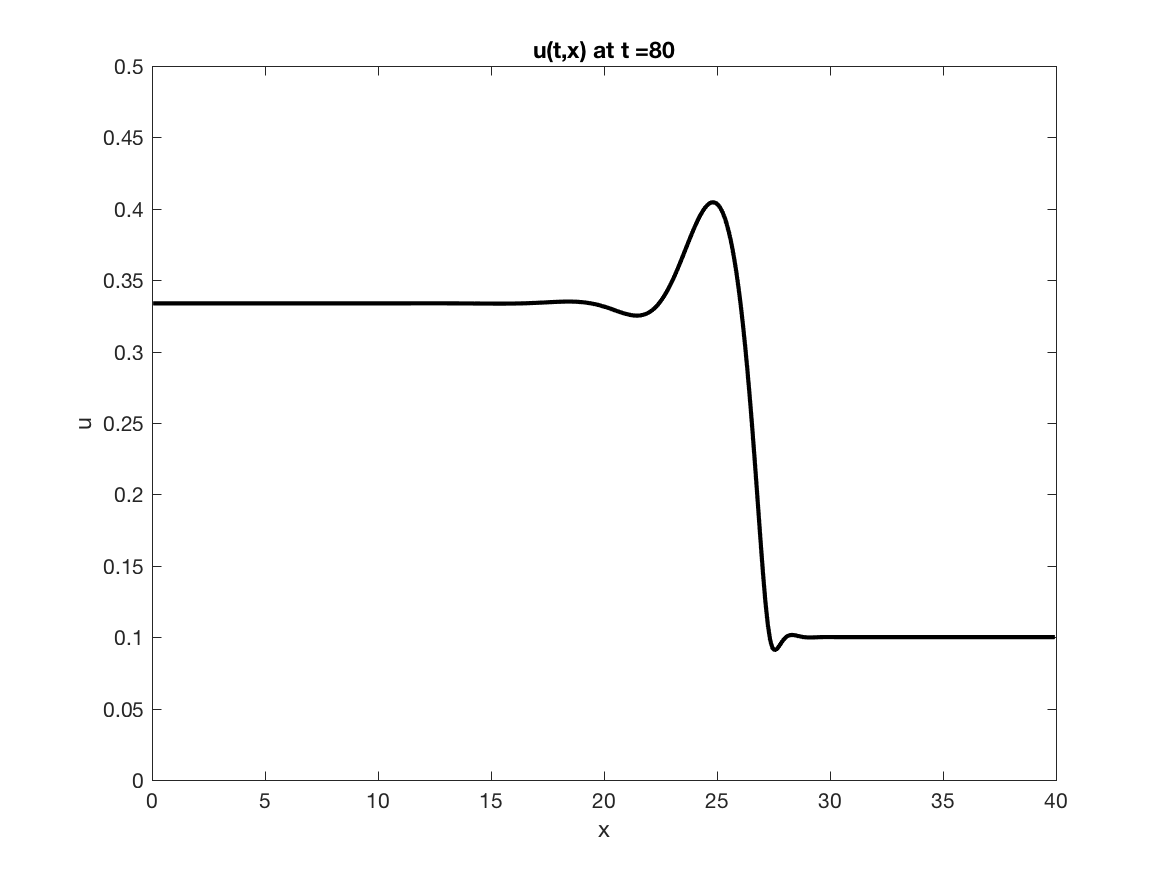
\includegraphics[scale=0.5]{Figures/reimann80.png}
      \end{center}
    \end{frame}
    \begin{frame}
      \frametitle{Numerical Results - Riemann Problem}
      \begin{center}
        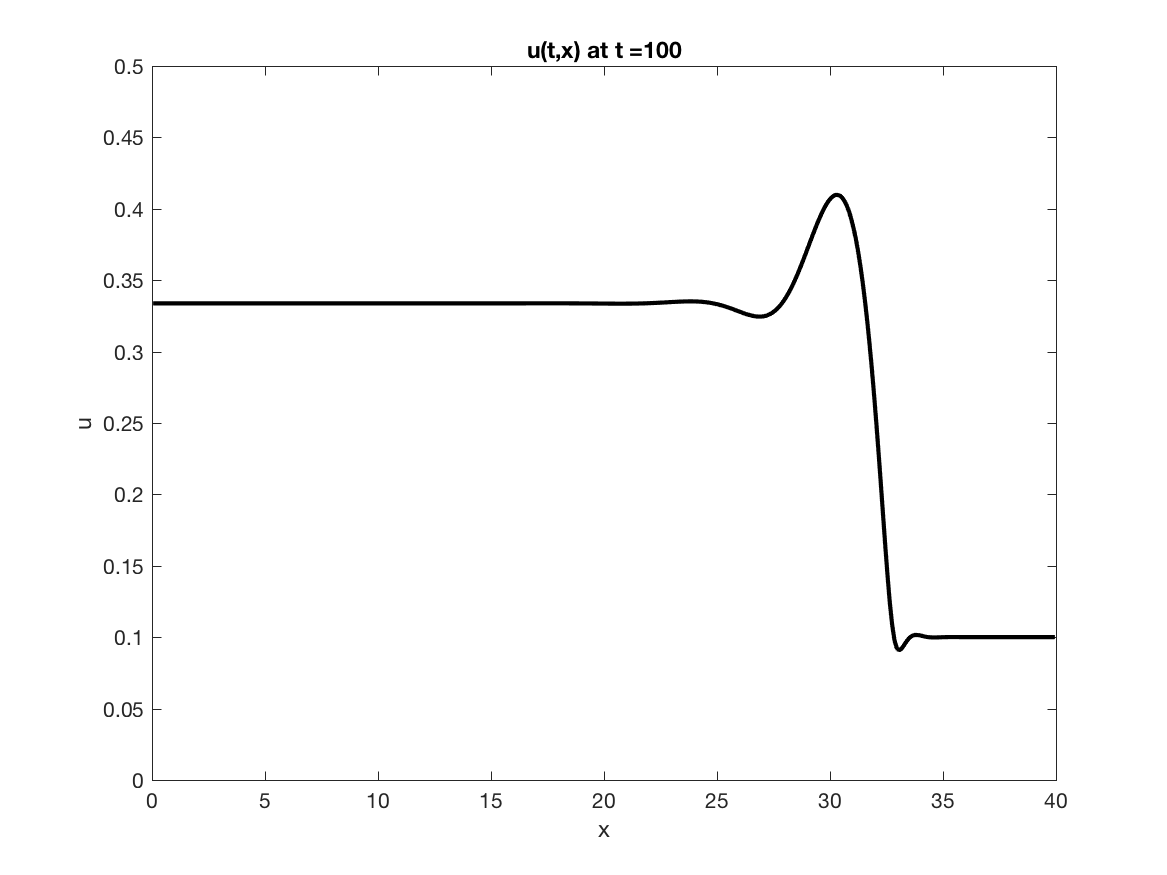
\includegraphics[scale=0.5]{Figures/reimann100.png}
      \end{center}
    \end{frame}

  \section{Conclusion}
    \begin{frame}
      \frametitle{Future Work}
      \begin{itemize}
        \item Higher dimensions
        \item Curved surfaces
        \item Space and time dependent coefficients
        \item Incorporation with air flow models
        \item Runge Kutta IMEX
      \end{itemize}
    \end{frame}

    \begin{frame}
      \frametitle{Conclusion}
      \begin{itemize}
        \item Thanks
          \begin{itemize}
            \item James Rossmanith
            \item Alric Rothmayer
          \end{itemize}
        \item Questions?
      \end{itemize}
    \end{frame}

    \begin{frame}
      \frametitle{Bibliography}
      % TODO: Bibliography
      \nocite{*}
      \printbibliography{}
    \end{frame}
\end{document}
